\section{Blockchain am Beispiel von Bitcoin}
Im Jahr 1991 haben Stuart Haber und W. Scott Stornetta mit ihrer Veröffentlichung \textit{How to Time-Stamp a Digital Document} die Grundlage für uns heute bekannte Blockchains gelegt. Durch Errechnen des Hashwertes eines Dokuments kann auch zu einem späteren Zeitpunkt belegt werden, dass ein Dokument nachträglich nicht verändert wurde. \cite{Haber.1991} 
\\
Darauf aufbauend wurde 2008 das Bitcoin Core Protokoll vorgestellt. Die grundlegende Idee ist es, Anwendern die Möglichkeit zu geben, Transaktionen ohne eine zentrale Institution abzuwickeln. Dazu führt jeder Teilnehmer eine eigene Historie über alle Transaktionen des Netzwerks. Sobald ein neuer Block generiert wurde, wird dieser an alle Teilnehmer des Netzwerks gesendet und in die Kette eingereiht. Dieses Kapitel beschreibt die Funktionsweise einer Proof of Work Blockchain am Beispiel von Bitcoin.

\subsection{Senden von Transaktionen}
Alle Anwender besitzen jeweils einen öffentlichen und einen privaten Schlüssel. Um eine Transaktion von einer Adresse senden zu können, muss der Sender sich mittels des privaten Schlüssels authentifizieren. Dazu signiert er die Transaktion, dargestellt in Formel \eqref{eq:signTransaction}. Es sei $s$ der private Schlüssel, $p$ der öffentliche Schlüssel und $t$ die zu signierende Transaktion.

\begin{equation}
sign(t, s) = Signatur
\label{eq:signTransaction}
\end{equation}

Die Transaktion wird zusammen mit der entstehenden Signatur an alle Teilnehmer des Netzwerks gesendet. Um zu bestätigen, dass einzig der Besitzer des privaten Schlüssels die Transaktion senden konnte, wird  die Korrektheit mittels Formel \eqref{eq:verifyTransaction} bestätigt.

\begin{equation}
verify(t, Signatur, p) = True/False
\label{eq:verifyTransaction}
\end{equation}

Das dezentrale Netzwerk kann so sicher sein, dass der zum öffentlichen Schlüssel passende private Schlüssel die Transaktion signiert hat.

Alice möchte nun 1 BTC an Bob senden. Sie signiert die Transaktion und sendet die entstehende Signatur zusammen mit ihrem öffentlichen Schlüssel und der auszuführenden Transaktion an alle Teilnehmer des Netzwerks. Um zu verhindern, dass Bob im Anschluss die gleiche Transaktion selbst mehrmals an das Netzwerk übermittelt und dadurch mehrere Transaktionen erhalten würde, wird zusätzlich eine eindeutige ID in der Transaktion festgelegt. \cite{Nakamoto.2009} \cite{Nielsen.2013} 

\subsection{Kryptografische Hash Funktion}
Die in Formel \eqref{eq:hashFunktion} dargestellte Funktion beschreibt eine kollisionsfreie Hashfunktion auf Bit-Ebene.
\begin{equation}
h : \{0,1\}^* \rightarrow \{0,1\}^l
\label{eq:hashFunktion}
\end{equation}

Eine beliebig lange Eingabe wird in eine vorgeschriebene Länge $l$ transformiert. Die Funktion $h$ besitzt darüber hinaus  folgende Eigenschaften:

\begin{enumerate}
 \item Funktion $h$ ist für einen Computer einfach zu berechnen
 \item Es ist unmöglich, dass für zwei verschiedene Eingaben $x$ und ${x}'$  das gleiche Ergebnis entsteht. Es gilt für alle $x$ und ${x}'$: $h(x) \neq h({x}')$
\end{enumerate}
\cite{Haber.1991}

\subsection{Generieren neuer Blöcke}
\label{sec:pow_section}
Alle neu entstehenden Transaktionen werden zu einem Block mit der maximalen Größe von 1 MB zusammengefasst. Etwa alle zehn Minuten entsteht ein solcher Block. Um die Transaktionen zu bestätigen, kann jeder Teilnehmer des Netzwerks selbst neue Blöcke errechnen. Ein Block gilt als gültig, wenn der Hashwert mit einer vom Netzwerk festgelegten Anzahl an vorausgehenden Nullen beginnt. Dazu wird aus dem Hashwert des vorherigen Blocks und den neu vorliegenden Transaktionen ein neuer Block gebildet. Zusätzlich wird eine Nonce im Block festgelegt. Dabei handelt es sich um eine zufällige Zahl, die aufgrund der bekannten Eigenschaften von Hashfunktionen den Hashwert des Blocks verändert. Die Teilnehmer berechnen den Hashwert mit verschiedenen Nonce-Werten, bis der Hashwert mit den vom Netzwerk festgelegten Anzahl an Nullen beginnt. Der Sachverhalt wird in Abbildung \eqref{fig:pow_valid_block} verdeutlicht. Sobald ein Teilnehmer eine solche Nonce gefunden hat, wird diese zusammen mit dem Block an das Netzwerk gesendet. Die anderen Teilnehmer können die Richtigkeit bestätigen. Dabei ist zu beachten, dass das Finden einer passenden Nonce komplett auf dem Zufall basiert. Als richtig markierte Blöcke werden in die Blockchain des Nutzers eingereiht. Jeder Nutzer führt seine eigene Blockhistorie. Zur Verdeutlichung soll Grafik \eqref{fig:Blockchain} dienen. \cite{Nielsen.2013}


\begin{figure}[h!]
    \centering
    \begin{minipage}{0.2\textwidth}
        \centering
        \begin{tikzpicture}
            \draw (0,0) rectangle (2,3) node[align=center, pos=.5] {
            $A \xrightarrow{\text{5}} B$\\
            $A \xrightarrow{\text{9}} C$\\ 
            <...>\\\\
            Nonce \\
            64392
            };
    \draw (0,1) rectangle (2,1);
    \draw (0,0) -- (1,-1) -- (2,0);    
    \node[draw] at (1,-1.5) {\textcolor{red}{3836253623673124}};
    \end{tikzpicture}
\end{minipage}\hfill
\begin{minipage}{0.2\textwidth}
\centering
\begin{tikzpicture}
            \draw (0,0) rectangle (2,3) node[align=center, pos=.5] {
            $A \xrightarrow{\text{5}} B$\\
            $A \xrightarrow{\text{9}} C$\\ 
            <...>\\\\
            Nonce \\
            94832
            };
    \draw (0,1) rectangle (2,1);
    \draw (0,0) -- (1,-1) -- (2,0);    
    \node[draw] at (1,-1.5) {\textcolor{green}{\textbf{00000000}23673124}};
    \end{tikzpicture}
    \end{minipage}
    \caption{Bildung des Hashwertes eines Blocks mit verschiedenen Nonce-Werten.} 
	\label{fig:pow_valid_block}
\end{figure}



\begin{figure}[h!]
	\includegraphics[width=1\linewidth]{images/blockchain_nonce_pdf_cropped}
	\caption{Vereinfachte Darstellung einer Blockchain. \cite{Nakamoto.2009}} 
	\label{fig:Blockchain}
\end{figure}

Da in jedem Block auf das vorherige Element referenziert wird, ist es unmöglich, zu einem späteren Zeitpunkt eine Änderung eine einem Block vorzunehmen oder die Reihenfolge der Blöcke zu ändern. Anzumerken ist, dass die Anforderung an die vorausgehenden Nullen stetig schwanken. Je mehr Nutzer nach Blöcken suchen, desto mehr Nullen werden benötigt. Im Umkehrschluss sinkt bei weniger Minern die Schwierigkeit. Dieses Verfahren wird als \textit{Proof of Work} (POW) bezeichnet.

\subsection{Die 51\%-Attacke als möglicher Angriff auf eine Proof of Work Blockchain}
\label{sec:51attack}
Ein potenzieller Angreifer, nennen wir ihn Mallory, möchte das Netzwerk manipulieren. Die Idee ist es, Bob 1 BTC zu senden, die Transaktion aber nur an Bob zu übertragen und vor den anderen Teilnehmern zu verheimlichen. Folglich hat nur Bob von dem Transfer erfahren und Mallory könnte zu einem späteren Zeitpunkt erneut über die Bitcoin verfügen und anderweitig ausgeben. Nach Absenden der Transaktion an Bob berechnet er eine wie in Abschnitt \eqref{sec:pow_section} dargestellte passende Nonce, sodass die vorangehenden Nullen der vom Netzwerk vorgegebenen Länge entsprechen. Findet Mallory eine passende Nonce, wird der neu erstellte Block an Bob gesendet. Parallel senden alle anderen Teilnehmer des Netzwerks ihre gefundenen  Blöcke an Bob. Da der von M gesendete Block nicht mit den anderen ankommenden Blöcken übereinstimmt, besitzt Bob zwei verschiedene Zustände des Netzwerks: Eine von Mallory manipulierte Version und die korrekte Blockkette. 
\\
Der Konsens besagt, dass in einem solchen Fall nur die längste Blockkette als korrekt anzusehen ist. Damit Bob die von Mallory manipulierte Version der Blockchain nicht verwirft, müsste Mallory konstant neue Blöcke erzeugen. Die Wahrscheinlichkeit, alleine mehr korrekte Blöcke finden zu können als das komplette Netzwerk, ist äußerst gering. Zu einem späteren Zeitpunkt wird Bob den manipulierten Fork des Netzwerks erkennen und verwerfen. Das beschriebene Problem wird als \textit{double-spending problem} bezeichnet. Um einen solchen Angriff auf das Netzwerk erfolgreich ausführen zu können, benötigt der Angreifer mindestens 51\% der Rechenleistung des Netzwerks. \cite{Yang.2019}

\subsection{Bewertung von Proof of Work}
In Abschnitt \eqref{sec:pow_section} wurde das Proof of Work Verfahren vorgestellt. Hinter jedem gefundenen Block steckt enormer Arbeitsaufwand in Form von Rechenleistung. Auf der einen Seite beweist das Finden einer passenden Nonce, dass der Block gültig und die in dem Block niedergeschriebenen Transaktionen ausgeführt wurden. Folglich ist eine spätere Manipulation ausgeschlossen. Auf der anderen Seite verbraucht das Suchen nach neuen Blöcken viel Energie. Je mehr Miner dem Netzwerk beitreten, desto schwieriger wird das Finden neuer Blöcke. Gleichzeitig ist das Netzwerk auf die in einen Block passenden Transaktionen beschränkt. Somit kann das Bitcoinprotokoll und ähnliche Proof of Work Blockchains unabhängig vom Energieverbrauch im Mittel etwa 5 Transaktionen pro Sekunde (TPS) verarbeiten. \cite{Cai.2019}

Über die Jahre hat sich Bitcoin als besonders sicher und dezentral bewiesen. Jeder kann am Netzwerk teilnehmen und die Dezentralität weiter vorantreiben. Dank sicherem POW ist seit Start der Blockchain kein erfolgreicher Angriff bekannt. Der anfallende Rechenaufwand muss in Kauf genommen werden, um das Netzwerk sicher fortführen zu können.